\documentclass{beamer}

\usetheme{GNURadio}
\usepackage{palatino}
\usepackage{xcolor}
\usepackage{tikz}
\usepackage[utf8]{inputenc}
\usepackage{listings}

\title{PyBOMBS \& CGRAN --- An Introduction}
\institute{Martin Braun}

\date{GNU Radio Conference 2016}

\graphicspath{{./}}
\DeclareGraphicsExtensions{.png,.pdf}

% Comment this out to not have a TOC every time you have a \section:
\AtBeginSection[] {%
  \begin{frame}
    \frametitle{Outline}
    \tableofcontents[currentsection]
  \end{frame}
}

\begin{document}

% Title page:
\frame{\titlepage}

\section{How do I even get started with GNU Radio?}
\begin{frame}
  \frametitle{Let's assume for just one minute\ldots}
  \begin{itemize}
    \item \ldots{}that I have no idea how to get started with GNU Radio.
    \item<2-> I mean, I literally don't even know how to run the examples and tutorials.
    \item<3-> No worries. We've got you covered.
  \end{itemize}
\end{frame}

\begin{frame}
  \frametitle{Top 4 easiest ways to install GNU Radio}
  \begin{enumerate}
    \item The GNU Radio Live DVD
    \item<2-> \texttt{apt-get install gnuradio} --- use your package manager, whatever that is
    \item<3-> PyBOMBS
    \item<4-> Source Builds
  \end{enumerate}
    \hspace{3em}
    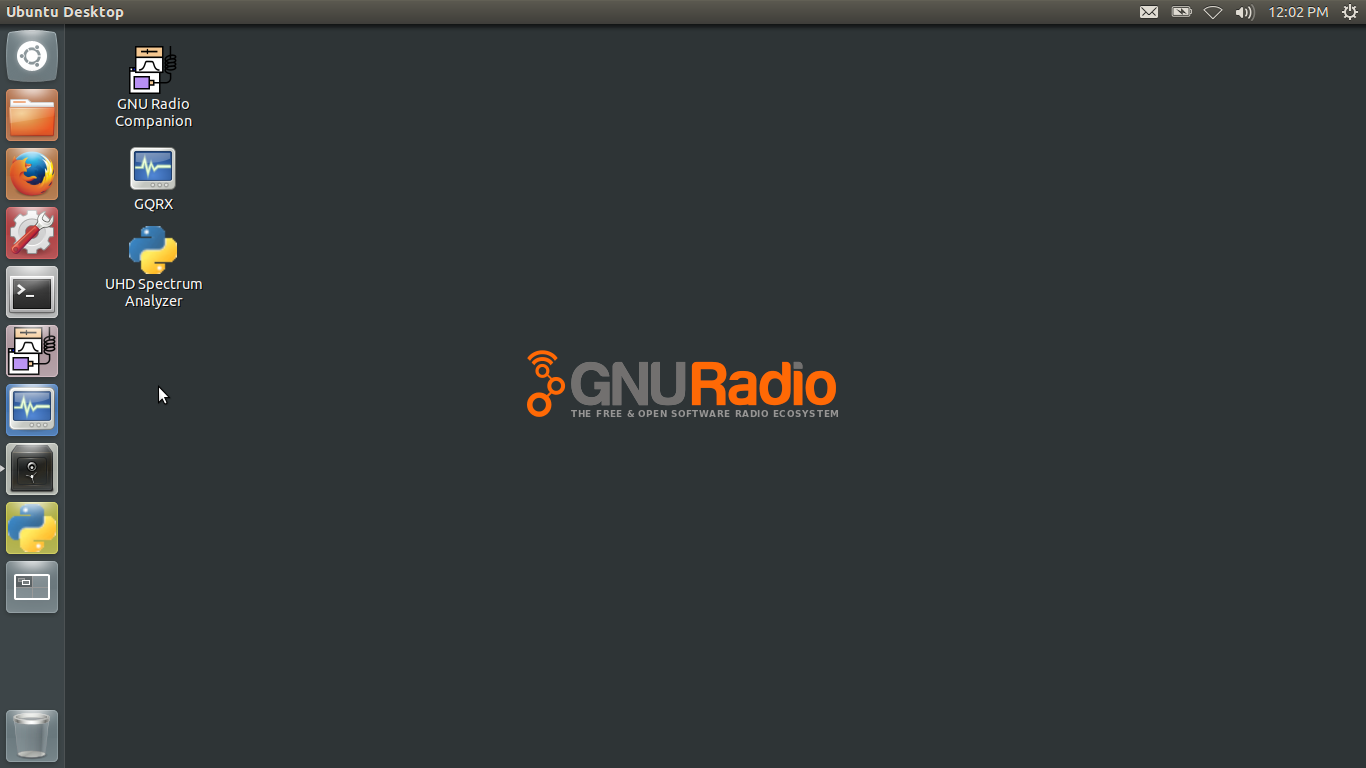
\includegraphics[height=5em]{grlivedvd}
    \hspace{1em}
    \includegraphics<3->[height=5em]{pybombs_logo}
    \hspace{1em}
    \includegraphics<4->[height=5em]{srcbuild}
\end{frame}

% Concepts:
% - Local prefix
% - 

\begin{frame}
  \frametitle{What you will need}
  \begin{itemize}
    \item A Linux or Mac box (one day we'll have Windows covered, but not today)
    \item Fedora, Ubuntu, CentOS, Debian, and probably many other distros fine
    \item Python 2.7
    \item<2-> And what else\ldots
    \item<3-> Nope, that's it!
  \end{itemize}
\end{frame}

\begin{frame}
  \frametitle{Getting started with PyBOMBS}
  \begin{itemize}
    \item Install PyBOMBS\@: \texttt{pip install pybombs}
    \item Optionally install PyBOMBS GUI\@: \texttt{pip install pybombs-qtgui}
    \item Let's just install GNU Radio and all major dependencies:
    \item \footnotesize{\texttt{pybombs prefix init -a default -R gnuradio-default /path/to/prefix/}}
  \end{itemize}
\end{frame}

%\section{Examples}
%\begin{frame}
  %\frametitle{Stuff}
  %\begin{block}{A Block's Title}
    %Math works too:
    %\begin{equation}
      %y(t) = x(t) * h(t)
    %\end{equation}
  %\end{block}
  %\begin{itemize}
    %\item foo
    %\item bar
    %\item baz
  %\end{itemize}
  %\begin{enumerate}
    %\item one
    %\item two
  %\end{enumerate}
%\end{frame}

\end{document}
